\documentclass[runningheads]{llncs}
\usepackage[T1]{fontenc}
\usepackage{algpseudocode, algorithm, amsmath, amssymb}					% packages to get the fonts, symbols used in most math
%\usepackage{dcolumn}
\usepackage[english]{babel}
\usepackage{hyperref}
\usepackage{multirow}
\usepackage{latexsym}
\usepackage{listings}
\usepackage{booktabs}
\usepackage{tabularx} % For dynamic table width
\usepackage{parcolumns}
\usepackage{subcaption} % For sub-listings
\newcolumntype{C}{>{\centering\arraybackslash}X}
\renewcommand{\arraystretch}{1.5}
\usepackage{pifont} % For check and cross symbols
\newcommand{\cmark}{\textcolor{darkgreen}{\ding{51}}}  % Checkmark
\newcommand{\xmark}{\textcolor{red}{\ding{55}}}  % Cross
\newcommand{\mmark}{\textcolor{orange}{\ding{106}}}  % Cross

% T1 fonts will be used to generate the final print and online PDFs,
% so please use T1 fonts in your manuscript whenever possible.
% Other font encondings may result in incorrect characters.
%
\usepackage{graphicx}
% Used for displaying a sample figure. If possible, figure files should
% be included in EPS format.
%
\usepackage{svg}
\usepackage[dvipsnames,svgnames, table]{xcolor} % text color
\DeclareFontFamily{U}{mathx}{\hyphenchar\font45}
\DeclareFontShape{U}{mathx}{m}{n}{
      <5> <6> <7> <8> <9> <10>
      <10.95> <12> <14.4> <17.28> <20.74> <24.88>
      mathx10
      }{}
\DeclareSymbolFont{mathx}{U}{mathx}{m}{n}
\DeclareMathSymbol{\bigtimes}{1}{mathx}{"91}

% Define a style for the listings
\lstset{
    basicstyle=\ttfamily\small,
    numbers=left,
    numberstyle=\tiny\color{gray},
    backgroundcolor=\color{lightgray!20},
    frame=single,
    captionpos=b,
    numbersep=5pt, % Adjust space between numbers and code
    % framexleftmargin=10pt,             % Extend frame margin for line numbers
}


\DeclareRobustCommand{\ojoin}{\rule[0.10ex]{.3em}{.4pt}\llap{\rule[1.40ex]{.3em}{.4pt}}}
\newcommand{\leftouterjoin}{\mathrel{\ojoin\mkern-6.5mu\Join}}
\newcommand{\rightouterjoin}{\mathrel{\Join\mkern-6.5mu\ojoin}}
\newcommand{\fullouterjoin}{\mathrel{\ojoin\mkern-6.5mu\Join\mkern-6.5mu\ojoin}}

\newcommand{\cormark}[1]{\textsuperscript{#1}}

\definecolor{eclipseStrings}{RGB}{42,0.0,255}
\definecolor{eclipseKeywords}{RGB}{127,0,85}
\definecolor{darkgreen}{RGB}{0,128,21}
\colorlet{numb}{magenta!60!black}
\setlength{\parskip}{0pt}

% Packages
\usepackage[normalem]{ulem} % wavy underlines
\makeatletter
\def\uwave{\bgroup \markoverwith{\lower3.5\p@\hbox{\sixly \textcolor{red}{\char58}}}\ULon}
\font\sixly=lasy6 % does not re-load if already loaded, so no memory problem.
\makeatother

% Comments
%\newcommand{\todo}[1]{\noindent\textcolor{red}{{\bf \{TODO}: #1{\bf \}}}}
\newcommand{\TODO}[1]{\todo{#1}}
\newcommand{\citeneeded}{\textcolor{red}{{\bf [?!]}}}
\newenvironment{draft}{\color{gray}}{\color{black}}
\newenvironment{changed}{\color{black}}{\color{black}}

% todonotes
\usepackage{xargs}                      % Use more than one optional parameter in a new commands
\usepackage[colorinlistoftodos,prependcaption,textsize=tiny]{todonotes}
\newcommandx{\unsure}[2][1=]{\todo[linecolor=red,backgroundcolor=red!25,bordercolor=red,#1]{#2}}
\newcommandx{\change}[2][1=]{\todo[linecolor=blue,backgroundcolor=blue!25,bordercolor=blue,#1]{#2}}
\newcommandx{\info}[2][1=]{\todo[linecolor=OliveGreen,backgroundcolor=OliveGreen!25,bordercolor=OliveGreen,#1]{#2}}
\newcommandx{\improvement}[2][1=]{\todo[linecolor=Plum,backgroundcolor=Plum!25,bordercolor=Plum,#1]{#2}}
\newcommandx{\thiswillnotshow}[2][1=]{\todo[disable,#1]{#2}}
\newcommandx{\todoi}[2][1=]{\todo[inline,size=\small,linecolor=Plum,backgroundcolor=Periwinkle!25,#1]{#2}}
\newcommandx{\todoCite}[2][1=]{\todo[linecolor=Plum,backgroundcolor=Periwinkle!25,bordercolor=Plum,#1]{#2}}
\newcommandx{\todoDef}[2][1=]{\todo[linecolor=Plum,backgroundcolor=Periwinkle!25,bordercolor=Plum,#1]{Def.: #2}}



% Reviewers
\newcommand\olaf[1]{{\color{RoyalBlue}\textbf{Olaf}: #1}}


% Annotations
\makeatletter
\font\uwavefont=lasyb10 scaled 700
\def\spelling{\bgroup\markoverwith{\lower3.5\p@\hbox{\uwavefont\textcolor{Red}{\char58}}}\ULon}
\def\grammar{\bgroup\markoverwith{\lower3.5\p@\hbox{\uwavefont\textcolor{LimeGreen}{\char58}}}\ULon}
\def\phrasing{\bgroup\markoverwith{\lower3.5\p@\hbox{\uwavefont\textcolor{blue}{\char58}}}\ULon}
\let\rephrase\phrasing
\newcommand\ins{\markoverwith{\textcolor{LimeGreen}{\rule[-0.5ex]{2pt}{0.4pt}}}\ULon}
\newcommand\remove{\bgroup\markoverwith{\textcolor{red}{\rule[0.5ex]{2pt}{0.4pt}}}\ULon}
\makeatother

\algrenewcommand\algorithmicrequire{\textbf{Input:}}
\algrenewcommand\algorithmicensure{\textbf{Returns:}}


\lstdefinelanguage{sparql}{
    basicstyle=\tiny,
    keywordstyle=\color{eclipseKeywords},
    commentstyle=\color{blue}, % style of comment
    stringstyle=\color{darkgreen},
    keywords={FILTER, NOT, EXISTS, bound, OPTIONAL, BIND, IF, isIRI, AS, INSERT, UPDATE, DELETE, WHERE, SELECT, UNION, rr,rml,ql,rdfs},
    morecomment=[n]{?}{\ },
    morecomment=[l]\#,
    morestring=[b]",
    morestring=[s]{<}{>},
    frame=lines,
}
\lstdefinelanguage{rdf}{
    basicstyle=\tiny,
    keywordstyle=\color{eclipseKeywords},
    commentstyle=\color{gray}, % style of comment
    stringstyle=\color{darkgreen},
    keywords={rml, ql, rr, rdfs},
    morecomment=[n]{?}{\ },
    morecomment=[l]\#,
    morestring=[b]",
    morestring=[s]{<}{>},
    frame=lines,
}


\lstdefinelanguage{triples}{
    basicstyle=\tiny,
    keywordstyle=\color{eclipseKeywords},
    commentstyle=\color{darkgreen}, % style of comment
    keywords={a, rml, ql, rr, rdfs},
    morecomment=[s]{?}{\ },
    frame=lines,
}

  

% Set symbols % 
\newcommand{\symFragmentUniverse}{\mathcal{F}}
\newcommand{\symAttrUniverse}{\mathcal{A}}
\newcommand{\symTermUniverse}{\mathcal{T}}
\newcommand{\symAllStrings}{\mathcal{S}} % the symbol for the set of all strings
\newcommand{\symAllIRIs}{\mathcal{I}} % the symbol for the set of all IRIs
\newcommand{\symAllLiterals}{\mathcal{L}} % the symbol for the set of all literals
\newcommand{\symAllBNodes}{\mathcal{B}} % the symbol for the set of all blank nodes
\newcommand{\symRMLGraph}{G}
\newcommand{\symDataObjUni}{\mathcal{D}}
\newcommand{\symDataAccUni}{\mathcal{Q}}
\newcommand{\symDataSeqUni}{\bar{\mathcal{O}}}
\newcommand{\symAttrSubSet}{A}
\newcommand{\symProjSet}{P}
\newcommand{\symMappingTupleSet}{M}
\newcommand{\symRenamePFunc}{R}
\newcommand{\bigDataObject}{D}
\newcommand{\symSetDataset}{\mathcal{D}^\texttt{\tiny ds}\!}
\newcommand{\symSetDatasetX}[1]{\mathcal{D}^\texttt{\tiny ds}_{#1}}
\newcommand{\symSetContentA}{\mathcal{D}^\texttt{\tiny c1}}
\newcommand{\symSetContentAX}[1]{\mathcal{D}^\texttt{\tiny c1}_{#1}}
\newcommand{\symSetContentB}{\mathcal{D}^\texttt{\tiny c2}}
\newcommand{\symSetContentBX}[1]{\mathcal{D}^\texttt{\tiny c2}_{#1}}
\newcommand{\symDataAcc}{L}
\newcommand{\symDataAccX}[1]{L_{#1}}
\newcommand{\symDataSeqCard}[1]{D^{seq,#1}}
\newcommand{\symAttrQueryMap}{\mathbb{P}}
\newcommand{\symDataSeq}{\bar{O}}
\newcommand{\symExtExprSet}{E}
\newcommand{\symExtExprSeq}{\bar{\symExtExprSet}}
\newcommand{\symExtPairs}{\symExtExprSet}
\newcommand{\symTermSeqUniverse}{\bar{\symTermUniverse}}
\newcommand{\symFragmentPFunc}{\bbbf}
\newcommand{\symFragmentSet}{F}
\newcommand{\symJoinAttrPairs}{\mathbb{J}}
\newcommand{\symExtFuncUni}{\mathcal{E}}

% Special values % 
\newcommand{\card}{card}
\newcommand{\fragAttr}{a_\mathrm{frag}}
\newcommand{\fragDefault}{f_{0}}
\newcommand{\attr}{a}
\newcommand{\subjAttr}{\attr_\textrm{s}}
\newcommand{\predAttr}{\attr_\textrm{p}}
\newcommand{\objAttr}{\attr_\textrm{o}}
\newcommand{\graphAttr}{\attr_\textrm{g}}
\newcommand{\fragment}[0]{fragment}
\newcommand{\error}{\epsilon}
\newcommand{\mappingTuple}{t}
\newcommand{\symMappingInst}{I}
\newcommand{\mappingRel}{(\symAttrSubSet, \symMappingInst)}
\newcommand{\mappingRelSpec}[1]{(\symAttrSubSet_{#1}, \symMappingInst_{#1})}
\newcommand{\queryExpr}{q}
\newcommand{\rootIt}{rit}
\newcommand{\cobit}{cobit}
\newcommand{\dataObject}{d}
\newcommand{\eval}{\mathit{eval}}
\newcommand{\evalX}[1]{\eval_{#1}}
\newcommand{\cbeval}{\mathit{eval}'\!}
\newcommand{\cbevalX}[1]{\eval_{#1}'}
\newcommand{\sourceType}{type}
\newcommand{\sourceTypeX}[1]{type_{#1}}
\newcommand{\sourceTypeTuple}{(\symSetDataset, \symSetContentA\!, \symSetContentB\!, \symDataAcc, \symDataAcc'\!, \eval, \cbeval, \typeCast)}
\newcommand{\sourceTypeTupleX}[1]{\sourceTypeTupleXXX{#1}{#1}{#1}}
\newcommand{\sourceTypeTupleXXX}[3]{(\symSetDatasetX{#1}, \symSetContentAX{#2}, \symSetContentBX{#3}, \symDataAccX{#2}, \symDataAccX{#3}', \evalX{#2}, \cbevalX{#3}, \typeCastX{#1})}
\newcommand{\dataSource}{s}
\newcommand{\dataSourceTuple}{(\sourceType,\bigDataObject)}
\newcommand{\iterConfig}{\bbbc}
\newcommand{\sourceOp}[3]{\textrm{Source}^{(#1,#2,#3)}}
\newcommand{\sourceOpDflt}{\sourceOp{\dataSource}{\queryExpr}{\symAttrQueryMap}}
\newcommand{\sourceOpTuple}{(\dataSource, \iterConfig)}
\newcommand{\attrQueryPair}{(\attr \rightarrow \queryExpr)}
\newcommand{\typeCast}{cast}
\newcommand{\typeCastX}[1]{\typeCast_{#1}}
\newcommand{\length}{len}
\newcommand{\var}{v}
\newcommand{\indexSeq}{M}
\newcommand{\extExpr}{\varphi}
\newcommand{\extEval}{eval}
\newcommand{\extPairsType}{(\symAttrUniverse \setminus \symAttrSubSet) \times \symExtExprSeqUni}
\newcommand{\serdeAttr}{a_{serialized}}
\newcommand{\bgp}{\bbbb}
\newcommand{\extFunc}{f}
\newcommand{\extFuncType}{(\symTermUniverse \cup \{\error\})}
\newcommand{\extFuncTuple}{(\extFunc,\extExpr_1,\dots,\extExpr_n)}
\newcommand{\extOp}{\text{Extend}_{\varphi}^{\attr}}
\newcommand{\extOpAttr}[1]{\text{Extend}_{\varphi}^{#1}}
\newcommand{\renameOp}{\text{Rename}^{\symRenamePFunc}}
\newcommand{\equiJoinOp}{\text{Join}^{\symJoinAttrPairs}_{=}}
\newcommand{\triplesMapIRI}{u}
\newcommand{\triplesMapGraph}[2]{\symRMLGraph_{#1}^{#2}}
\newcommand{\toIRI}{\texttt{toIRI}}
\newcommand{\toBNode}{\texttt{toBNode}^{\LTB}}
\newcommand{\toLiteral}{\texttt{toLiteral}}
\newcommand{\template}{\texttt{template}^{\symAttrQueryMap}}
\newcommand{\initSrc}{\texttt{initSrc}}
\newcommand{\concat}{\texttt{concat}}
\newcommand{\concatSeq}{\texttt{concatSeq}}
\newcommand{\literal}{\ell}
\newcommand{\lex}{\mathit{lex}}
\newcommand{\dt}{\mathit{dt}}
\newcommand{\literalTuple}{(\lex, \dt)}
\newcommand{\LTB}{\mathit{L2B}}
\newcommand{\tempSubStrs}{\texttt{tempSubStrs}}
\newcommand{\substrSeq}{\bar{S}}
\newcommand{\projectOp}[1]{\text{Project}^{#1}}
\newcommand{\natJoin}{\text{NatJoin}}
\newcommand{\union}{\text{Union}}

% Functions % 
\newcommand{\fctDom}[1]{\mathrm{dom}(#1)}
\newcommand{\fctMappingTuple}[1]{\mappingTuple(#1)}
\newcommand{\fctAttrs}[1]{\mathrm{attrs}(#1)}
\newcommand{\fctCard}[2]{\card[#1](#2)}
\newcommand{\fctRootIt}[2]{\rootIt(#1, #2)}
\newcommand{\fctCobit}[3]{\cobit(#1, #2, #3)}
\newcommand{\fctEval}[2]{\eval(#1,#2)}
\newcommand{\fctEvalLang}[3]{\eval^{#3}(#1,#2)}
\newcommand{\fctCbeval}[3]{\cbeval(#1,#2,#3)}
\newcommand{\fctCbevalLang}[4]{\cbeval^{#4}(#1,#2,#3)}
\newcommand{\fctTypeCast}[1]{\typeCast(#1)}
\newcommand{\fctLength}[1]{\length(#1)}
\newcommand{\fctRenameTuple}[2]{rename^{#1}(#2)}
\newcommand{\fctSubst}[2]{subst^{#1}(#2)}
\newcommand{\fctExtFuncEvalN}[2]{\extFunc(\fctEval{#1_1}{#2},\dots,\fctEval{#1_n}{#2})}
\newcommand{\fctExtOp}[1]{\extOp(#1)}
\newcommand{\fctExtOpBig}[1]{\extOp\bigl(#1\bigr)}
\newcommand{\fctExtOpX}[3]{\text{Extend}^{#1}_{#2}(#3)}
\newcommand{\fctExtOpXBig}[3]{\text{Extend}^{#1}_{#2}\bigl(#3\bigr)}
\newcommand{\fctRenameOp}[1]{\renameOp(#1)}
\newcommand{\fctRenameOpBig}[1]{\renameOp\bigl(#1\bigr)}
\newcommand{\fctEquiJoinOp}[2]{\equiJoinOp(#1, #2)}
\newcommand{\fctEquiJoinOpBig}[2]{\equiJoinOp\bigl(#1, #2\bigr)}
\newcommand{\fctToIRI}[1]{\toIRI(#1)}
\newcommand{\fctToBNode}[1]{\toBNode(#1)}
\newcommand{\fctToLiteral}[1]{\toLiteral(#1)}
\newcommand{\fctTemplate}[1]{\template(#1)}
\newcommand{\fctImg}[1]{\mathrm{img}(#1)}
\newcommand{\fctInitSrc}[1]{\initSrc(#1)}
\newcommand{\fctConcat}[2]{\concat(#1, #2)}
\newcommand{\fctConcatSeq}[1]{\concatSeq(#1)}
\newcommand{\fctTempSubStrs}[1]{\tempSubStrs(#1)}
\newcommand{\fctProjectOpDflt}[1]{\fctProjectOp{\symProjSet}{#1}}
\newcommand{\fctProjectOp}[2]{\projectOp{#1}(#2)}
\newcommand{\fctProjectOpBig}[2]{\projectOp{#1}\bigl(#2\bigr)}
\newcommand{\fctNatJoin}[2]{\natJoin(#1,#2)}
\newcommand{\fctUnion}[2]{\union(#1,#2)}

% Layout %
\newcommand{\ttl}[1]{\texttt{\small #1}}  % for conrete IRIs, etc. used in examples and in formulas



%%%%%%%%%%%%%%%%%%%%%%%%%%%%%%%%%%%%%%%%%%%%%%%
% The following ensures that we have a (non-visible) table of contents embedded
% in the PDF, which PDF readers can show and, thus, allows me to navigate the
% document more easily.
%                                    Olaf
\setcounter{tocdepth}{3}
\hypersetup{bookmarksopen=true, citecolor=blue}
%
%%%%%%%%%%%%%%%%%%%%%%%%%%%%%%%%%%%%%%%%%%%%%%%


\begin{document}												% end of preamble and beginning of text that will be printed

\title{The Semantic Web Language Server: enhancing the developer experience for Semantic Web practitioners}
%
%\titlerunning{Abbreviated paper title}
% If the paper title is too long for the running head, you can set
% an abbreviated paper title here
%
\author{Arthur Vercruysse\inst{1}\orcidID{0000-0003-3467-9755} \and
Julián {Rojas Meléndez}\inst{1}\orcidID{0000-0002-6645-1264} \and 
Pieter Colpaert\inst{1}\orcidID{0000-0001-6917-2167}}
%

\titlerunning{The Semantic Web Language Server}
\authorrunning{A. Vercruysse et al.}
% First names are abbreviated in the running head.
% If there are more than two authors, 'et al.' is used.
%
\institute{
IDLab, Department of Electronics and Information Systems, Ghent University -- imec \\
\email{firstname.lastname@ugent.be}}
%
\maketitle              % typeset the header of the contribution
%
% \begin{abstract}
% % Context (What is needed to understand the "need"?)
%   The semantic web has produced many syntaxes to interact with it: from data format to querying to reasoning.
% % Need (Why something needed to be done at all?)
%   These formats all suffer from human imprecisions, a single typo changes the entire semantics of the document, leaving it non-interoperable.
% % Task (What was undertaken to address the need? It’s here that you write ‘in this paper, we …’)
%   In this paper, we introduce the semantic language server.
% % Object (What the present document does or covers)
%   The language server enhances semantic documents with IDE functionality. 
%   Notifying the users early about potential mistakes from typo's to SHACL violations.
% % Findings (What the work done yielded or revealed)
%   By combining and extending the state of the art, we enhanced the efficienty, precision and confidance of end users working with semantic documents,
%   including power users, newcomers, domain experts and data engineers.
% % Conclusion (What the findings mean for the audience)
%   With the semantic language server users can expect the similar functionality as existing tools like Yasgui, but closer the user in their coding environment.
% % Perspectives (What the future holds, beyond this work)
% \keywords{Language Server, IDE, Tool}
% \end{abstract}


\begin{abstract}
% Context (What is needed to understand the "need"?)
The semantic web has introduced a variety of syntaxes for data representation, querying, and reasoning, such as Turtle, SPARQL, and SHACL.
% Need (Why something needed to be done at all?)
While these formats enable powerful interactions with linked data, they are highly sensitive to human errors; even minor typos can disrupt the semantics of a document, rendering it invalid or non-interoperable.
% Task (What was undertaken to address the need? It’s here that you write ‘in this paper, we …’)
In this paper, we present the Semantic Language Server, a tool designed to enhance the editing experience for semantic web documents by integrating IDE functionalities directly into the user's coding environment.
% Object (What the present document does or covers)
The language server provides features such as real-time syntax validation, autocompletion, and SHACL-based diagnostics to notify users of potential mistakes early in the development process.
The language server is available as extensions for popular platforms like VS Code and Neovim, as well as in a standalone web-based interface (integrated into a Monaco editor).
% Findings (What the work done yielded or revealed)
By building on and extending the state of the art, our tool improves the efficiency, precision, and confidence of various user groups, including semantic power users, newcomers, domain experts, and data engineers.
% Conclusion (What the findings mean for the audience)
Semantic Language Server offers comparable functionality to existing tools like YASGUI but with greater accessibility and integration into familiar development workflows. 
% Perspectives (What the future holds, beyond this work)
This work not only addresses current limitations in semantic web tooling but also paves the way for broader adoption of semantic technologies by reducing barriers and improving usability.
\keywords{Language Server, IDE, Tool}
\end{abstract}

\section{Introduction}%
\label{sec:introduction}

% Enhancing semantic web adoption by lowering the barrier to learn (ref Two Decades On)
% In this paper we introduce Semantic LSP, a language server to bring enhanced editing linked data documents, including turtle, jsonld and sparql.

% Focus not only on semantic engineers, people that work daily with semantic data
% But also focus on data engineers that create intriguing sparql queries over the precious semantic data
% Focus also on the domain experts, sometimes installing extra software is too big a hurdle
% These people we call 'end users' (cite  10.1145/1922649.1922658)

% End users should focus on the following steps
% - Requirements: How the software should behave in the world
% - Design and specifications: How the software behaves internally to achieve the requirements
% - Reuse: Using preexisting code to save time and avoid errors (including integration, extension, and other perfective maintenance)
% - Testing and Verification: Gaining confidence about correctness and identifying failures.
% - Debugging: Repairing known failures by locating and correcting errors.
% Language servers help the end user with design and reuse by bringing autocompletion to the editor. 
% Design is more fluent for the domain experts because writing OWL and RDFS is faster and less error prone.
% Reuse is stimulated by already suggesting defined properties when writing turtle.
% Testing and verification is enhanced by using SHACL shapes to valide user data on the fly and ensuring correct syntax.

% A language server also serves to lowering the barrier to active learning. Users in the study ... et al attested to the complexity of creating sparql queryies for wikidata.
% Autocompletion on properties and suggesting properties with plain texts help the students explore the ontology and lets them create more intriguing queries.


% There is already a lot of related work, even in the area of the semantic web (cite yasgui).
% Yasgui showed that lowering the barrier to entry indeed does encourage more usage and raised the semantic literacie quite quickly.
% We believe that taking those concepts and expanding on them to support more semantic languages and focussing on a easy to use design that promotes extensibily is a great oportunity to advance the state of the art.

The Semantic Web has matured over the past two decades, yet its broad adoption remains a challenge.
One of main critiques appears to be the usability of the technology and its accessibility to newcomers~\cite{10.3233/SW-190387}. 
It is difficult for users across varying levels of expertise to effectively create, manage, and query semantic data, which we attribute to a lack of tooling.
This need becomes evident when considering the distinct challenges faced by key user groups:

\begin{enumerate}
  \item \textbf{Semantic Power Users}\\
    Experienced semantic engineers require advanced tools to efficiently manage large datasets, develop ontologies, and perform reasoning tasks.
    While proficient, even these users benefit from features that reduce cognitive overhead, minimize manual errors, and accelerate routine operations.
    % PC: Next sentence commented: too early - this is not a saled pith!
    %Tools like Semantic LSP provide real-time feedback, context-aware autocompletion, and error diagnostics, significantly streamlining their workflows.

  \item \textbf{Newcomers and Casual Users}\\
    Beginners, including students and hobbyists, often struggle with the intricacies of semantic technologies~\cite{EvensteinSigalov2023,Turki2021RepresentingCI}. 
    Writing valid RDF documents or crafting correct SPARQL queries can be overwhelming without proper guidance. 
    % PC: too early
    %Semantic LSP supports active learning by offering user-friendly features such as syntax highlighting, contextual autocompletion, and hover-based documentation, empowering newcomers to experiment confidently and overcome the steep learning curve.

\item \textbf{Domain Experts Creating Ontologies}\\
    Domain experts typically rely on tools like Protégé for ontology creation. 
    However, such tools can introduce bottlenecks, particularly for smaller projects, due to setup complexity and steep learning curves. 
    %Semantic LSP offers a lightweight alternative by enabling ontology creation directly within text editors using Turtle.
    %This approach is especially beneficial for quick iterations and avoids the overhead of additional software installation and configuration.

  \item \textbf{Data Engineers Crafting SPARQL Queries}\\
    Data engineers frequently face challenges in exploring unfamiliar ontologies and writing sophisticated queries. 
    %Semantic LSP facilitates these tasks with intelligent autocompletion, which suggests properties and classes based on context, and hover-based explanations that help users understand ontology structures.
    %These features reduce errors, improve query quality, and promote deeper engagement with semantic data.
\end{enumerate}

Integrated Development Environments (IDEs) are widely recognized for their ability to improve developer productivity, streamline workflows, and reduce common mistakes across various domains~\cite{javaEngineer}. 
Features like syntax highlighting and diagnostics are not merely conveniences; they are essential tools for ensuring accuracy and maintaining consistency. 
In recent years, the Language Server Protocol has been standardized\footnote{\url{https://microsoft.github.io/language-server-protocol/}} and implemented in most IDEs to provide such features independent of a specific IDE.
For example, Visual Studio Code, Neovim or event the web-based Monaco editor can in this way be extended with language-specific functionalities by coding a Language Server only once.
%Despite these benefits, such productivity-enhancing features are underrepresented in semantic web tooling.

To address the challenges faces by our key user groups, we introduce the Semantic Web Language Server (SWLS).
This is a language server designed to enhance the editing experience specifically for linked data documents. 
For power users, SWLS intends to provide real-time feedback, context-aware autocompletion, and error diagnostics, significantly streamlining their workflows.
For newcomers, SWLS aims to supports active learning by offering user-friendly features such as syntax highlighting, contextual autocompletion, and hover-based documentation, empowering newcomers to experiment confidently and overcome the steep learning curve.
For domain experts, SWLS wants to offer a lightweight alternative to for example Protégé, by enabling ontology creation directly within text editors using Turtle.
This approach is especially beneficial for quick iterations and avoids the overhead of additional software installation and configuration.
Finally, for data engineers crafting SPARQL queries, SWLS intends to help them with intelligent autocompletion, which suggests properties and classes based on context, and hover-based explanations that help users understand ontology structures.
These features reduce errors, improve query quality, and promote deeper engagement with semantic data.

%By leveraging features such as autocompletion, diagnostics, and real-time validation, Semantic LSP aims to lower the barriers to semantic web adoption while improving productivity and reducing common errors.

Previous efforts, such as YASGUI for SPARQL query editing, have shown the value of lowering entry barriers by improving usability~\cite{10.3233/SW-150197,10.1007/978-3-642-41242-4_7}. 
SWLS builds on these successes, expanding support to multiple semantic languages and emphasizing a user-friendly, extensible design. 
By addressing the needs of our user groups, we aim to advance the state of the art in Semantic Web tooling and encourage broader adoption.

We start with a study of the state of the art in tooling currently available to our user groups.
We then introduce the SWLS and run over its capabilities and how this has been implemented.
\todo{Finally, we elaborate ...}

\section{Related Work}%
\label{sec:related_work}

In this section we look at the related state of the art.
The state of the art is full of different implementations that handle some specific part of the semantic web.
From ontology designers like protege to Yasgui's sparql query editors.
This section covers the different IDE functionalities that can be implemented for the semantic web, Table 1 provides details on current and open-source implementations that implement parts of these functionalities.

\paragraph*{Highlighting}

Highlighting helps human brains parse data more easily.
There are two different parts of highlighting: syntactic highlighting and semantic highlighting.
The former only concerns itself with the syntax of a document. A lexer can handle this highlighting very effectively and allows for example to hightlight strings as green and namednodes as red.
Semnatic highlighting on the other hand can use document semantics. Semantics can be for example the term kind of a term, only inferable by extracting the actual triples or marking the type of an object in a different colour.

Please note that undefined properties etc should not be highlighed differently by the semantic highlighter, undefined properties should be handled as diagnostics.


\paragraph*{Diagnostics}

Diagnostics are of utmost importance, nothing is more draining than to check whether or not some data is correctly written at runtime.
The editor should be able to notify the user that the current document would not be parsed by parsers following the standard.

Other diagnostics are also very relevant and can inform the user that the current data may not be what they expect.
For example the editor can notify the user when an undefined property is used, alerting the user that it could be a typo.
The editor can also notify the user about reasoning mistakes, when creating an ontology or creating data that should adhere to an ontology or to a SHACL shape.


\paragraph*{Formatting}

It is expected that an IDE helps the developer to keep a consistent format over different documents, again helping the user parse the data more effectively.
Formatting however is a subjective matter and should be configurable by the user or codebase.

\paragraph*{Renaming}
Often an editor allows the user to rename identifiers as a quality of life improvemt.
This allows the user to more easily iterate over data and aliviating the writer's block.


\paragraph*{Completion}

Completion comes again in two flavours: completing keywords and already defined tokens and semantic completion.
Semantic completion can complete with defined properties and defined classes and can check the current context of the completion, answering the question "Is the user current writing a class or a property?".

Naive completion can suggest all defined properties and defined classes but this is not always wanted, the editor should also be able to derive the type of the current subject for example and only suggest properties that are defined with that type as domain.
On the other hand when the user is writing an object, the editor can also suggest already defined entities that have the correct type checking the range of the property.



% we might want to transpose the headers
\begin{table}[h!]
    \centering
  \begin{tabularx}{\textwidth}{ |p{3cm}|C|C|C|C|C|C|C|C|C|C|C|C|}
\hline
    \multirow{2}{*}{} & \multicolumn{2}{c|}{Highlight} & \multicolumn{3}{c|}{Diagnostics} & \multicolumn{4}{c|}{Completion}  & \multirow{2}{*}{} & \multirow{2}{*}{} & \multirow{2}{*}{} \\ \cline{2-10} 

      LSP implementation                & \rotatebox{90}{Syntactic} & \rotatebox{90}{Semantic} %highlighting
                                        & \rotatebox{90}{Syntax} & \rotatebox{90}{Undefined} & \rotatebox{90}{Validation\ \ }  %diagnostics
                                        & \rotatebox{90}{Syntax} & \rotatebox{90}{Tokens} & \rotatebox{90}{Naieve} & \rotatebox{90}{Typed} % completion
                                        & \rotatebox{90}{Formatting} 
                                        & \rotatebox{90}{Renaming}
                                        & \rotatebox{90}{Polyglot} \\ \hline
Stardog                       & \cmark & \xmark & \cmark & \xmark & \xmark & \cmark & \cmark & \mmark & \xmark & \xmark & \xmark & \cmark \\
RDFox                         & \cmark & \xmark & \xmark & \xmark & \xmark & \mmark & \xmark & \xmark & \xmark & \xmark & \xmark & \cmark \\
query.wikidata                & \cmark & \xmark & \xmark & \xmark & \xmark & \xmark & \cmark & \cmark & \xmark & \xmark & \xmark & \xmark \\
yasgui                        & \cmark & \xmark & \cmark & \xmark & \xmark & \xmark & \cmark & \cmark & \xmark & \xmark & \xmark & \xmark \\
Protege                       & N/A    & N/A    & N/A    & N/A    & \cmark & N/A    & \cmark & N/A    & N/A    & N/A    & \cmark & \xmark \\
rdf-vocabularies-autocomplete & \xmark & \xmark & \xmark & \xmark & \xmark & \xmark & \xmark & \cmark & \xmark & \xmark & \xmark & \xmark \\
\hline
\end{tabularx}
    \caption{\label{tab:current_implementations}Table without predefining column count explicitly. Stardog simple completion is based on a fixed list of items. RDFox syntax completion only works for SPARQL functions.}
\end{table}


\subsection*{Some words on ontology designing tools}
Their main helping functions\cite{ComparingOntologyBuildingTools}.

\subsection{Language Server Protocol}

Language Servers using the Language Server Protocol\cite{IntroToLsp} 
are cool \cite{GLSPFlexibility}.



%% GPT

\section{Related Work}%
\label{sec:related_work}

This section examines the state of the art in tools and functionalities for semantic web development. 
Current implementations address various aspects of semantic web technologies, ranging from ontology modeling tools like Protégé to SPARQL query editors such as YASGUI.
While these tools provide specialized capabilities, the integration of features typical of Integrated Development Environments (IDEs) remains limited. 
Table~\ref{tab:current_implementations} summarizes open-source tools that implement selected IDE functionalities for semantic web technologies.

\paragraph*{Highlighting} enhances readability by leveraging visual cues, which assist developers in parsing complex data. 

There are two primary types of highlighting: \textbf{syntactic} and \textbf{semantic}.
\begin{itemize}
    \item \textbf{Syntactic highlighting} focuses on document syntax and is implemented using lexers. For example, strings might appear in green, while named nodes are highlighted in red. This type of highlighting does not require knowledge of the document’s meaning.
    \item \textbf{Semantic highlighting}, in contrast, uses document semantics to differentiate terms based on their roles. For instance, the type of an object could be highlighted in a unique color, or terms inferred from triples could be visually distinguished.
\end{itemize}
Semantic highlighters should avoid overloading the user with unnecessary information. Undefined properties, for example, should not be highlighted differently; such cases are better addressed by diagnostic features.


\paragraph*{Diagnostics} are essential for identifying issues early in the development process. 
Rather than deferring error detection to runtime, an IDE should provide immediate feedback on data validity.

Examples of valuable diagnostics include:
\begin{itemize}
    \item \textbf{Standard compliance}: Notifying users if the current document is incompatible with parsers adhering to semantic web standards.
    \item \textbf{Undefined properties}: Alerting users to potential typos or incorrect terms when undefined properties are detected.
    \item \textbf{Reasoning errors}: Highlighting logical inconsistencies in ontologies or data that deviate from expected SHACL shapes or OWL reasoning.
\end{itemize}

These features enable developers to maintain data accuracy and reduce time spent debugging.


\paragraph*{Formatting}

Consistent formatting across documents enhances readability and maintainability.
An IDE should assist users in adhering to a defined style guide while allowing customization to accommodate different workflows or preferences.

\paragraph*{Renaming} identifiers, such as classes or properties, is a critical feature for iterative development.
This functionality helps users manage data more efficiently and adapt to evolving project requirements without introducing errors.

\paragraph*{Completion} features, like highlighting, can be categorized as \textbf{syntactic} or \textbf{semantic}:

\begin{itemize}
    \item \textbf{Syntactic completion} involves suggesting keywords or tokens already defined in the document.
    \item \textbf{Semantic completion} provides context-aware suggestions, such as properties or classes relevant to the current position. For example:
    \begin{itemize}
        \item When writing a property, the IDE can suggest those defined for the subject's type.
        \item When completing an object, it can suggest entities consistent with the property's range.
    \end{itemize}
\end{itemize}

Naive completion might suggest all possible terms, but a sophisticated system should filter suggestions based on the context, such as the inferred type of the current subject or object.


\subsection*{Ontology Design Tools}

Ontology design tools, such as Protégé, serve as the foundation for many semantic web development workflows. 
Their primary functions include visualizing ontologies, defining classes and properties, and validating logical consistency.
These tools provide essential support but often lack the integrated functionality of modern IDEs, such as context-aware diagnostics or advanced refactoring capabilities~\cite{ComparingOntologyBuildingTools}.



\section{Semantic LSP}%
\label{sec:semantic_lsp}

During the development of the Semantic Language Server (SLS), we adhered to state-of-the-art implementation practices to ensure modularity, scalability, and maintainability\cite{10.1145/3550355.3552452,10.1145/3563834.3567537,10.1145/3550355.3552452,Bour_2018}.
Unlike traditional architectures, SLS leverages an entity component system (ECS), which offers greater separation of concerns compared to the widely recognized \textit{Layered Architecture}\cite{10.1145/3550355.3552452}.

\todo{Add information about Resources}
An ECS is a software design pattern that organizes a program into four key elements: Entities, Components, Systems, and Resources. 
In SLS, entities represent documents that are composed of various components. 
Components store data associated with the entity, such as the document's contents, file location, or derived RDF triples. 
Systems are functions designed to process specific components and are grouped into schedules to achieve distinct tasks. 
For example, the \textit{Parse} schedule includes systems responsible for tokenization, parsing, and triple extraction.
Semantic languages integrate seamlessly by introducing their systems into these predefined schedules to provide language-specific functionality.

As noted by Bour et al., "No spec, no tests" highlights the challenge of developing test suites for user-facing applications like language servers, where specifications can be open to interpretation\cite{Bour_2018}. 
To address this, SLS implements shared systems for common functionality, ensuring consistency and reducing redundancy across various semantic web languages.
By adopting this approach, SLS delivers uniform features, while maintaining flexibility for language-specific extensions.

SLS is implemented in Rust and leverages Bevy’s Entity Component System (ECS) to maintain a highly modular and efficient architecture.
Features are typically added in two steps:
  first, extracting the necessary data from RDF triples and attaching it to relevant entities; 
  second, using this data to implement language server functionalities such as diagnostics or autocompletion.

Bevy ECS facilitates this process by allowing the creation of isolated components and systems, enabling new features to be developed without impacting existing functionality.
This modularity ensures that only the minimal required data is extracted for each task, avoiding the complexity and overhead of constructing a complete digital twin of the dataset.

For example, to implement autocompletion based on defined classes, two small systems are added:
  one to extract information about defined classes and their descriptions,
  and another to incorporate this information into autocompletion requests. 
Similarly, adding a feature to display type hierarchies would involve creating a system to extract data specific to the rdfs:subclassOf relation, without interfering with other systems.
This approach allows for scalable and focused development of language server features.


\subsection{Langauge Server schedules}

This section details the systems implemented within each schedule of the Semantic Language Server (SLS).
Some systems are designed primarily to generate components, which are then utilized by other systems, potentially across different schedules.
This decoupled design ensures flexibility and modularity. 
If a system expects a component that is not present for a given entity, the system simply skips that entity.
This behavior supports asynchronous execution of systems, allowing for independent processing and reducing bottlenecks in the language server’s operation.

\subsubsection{Parse}

\begin{figure}[tb]
 \centering
 \makebox[\textwidth]{%
    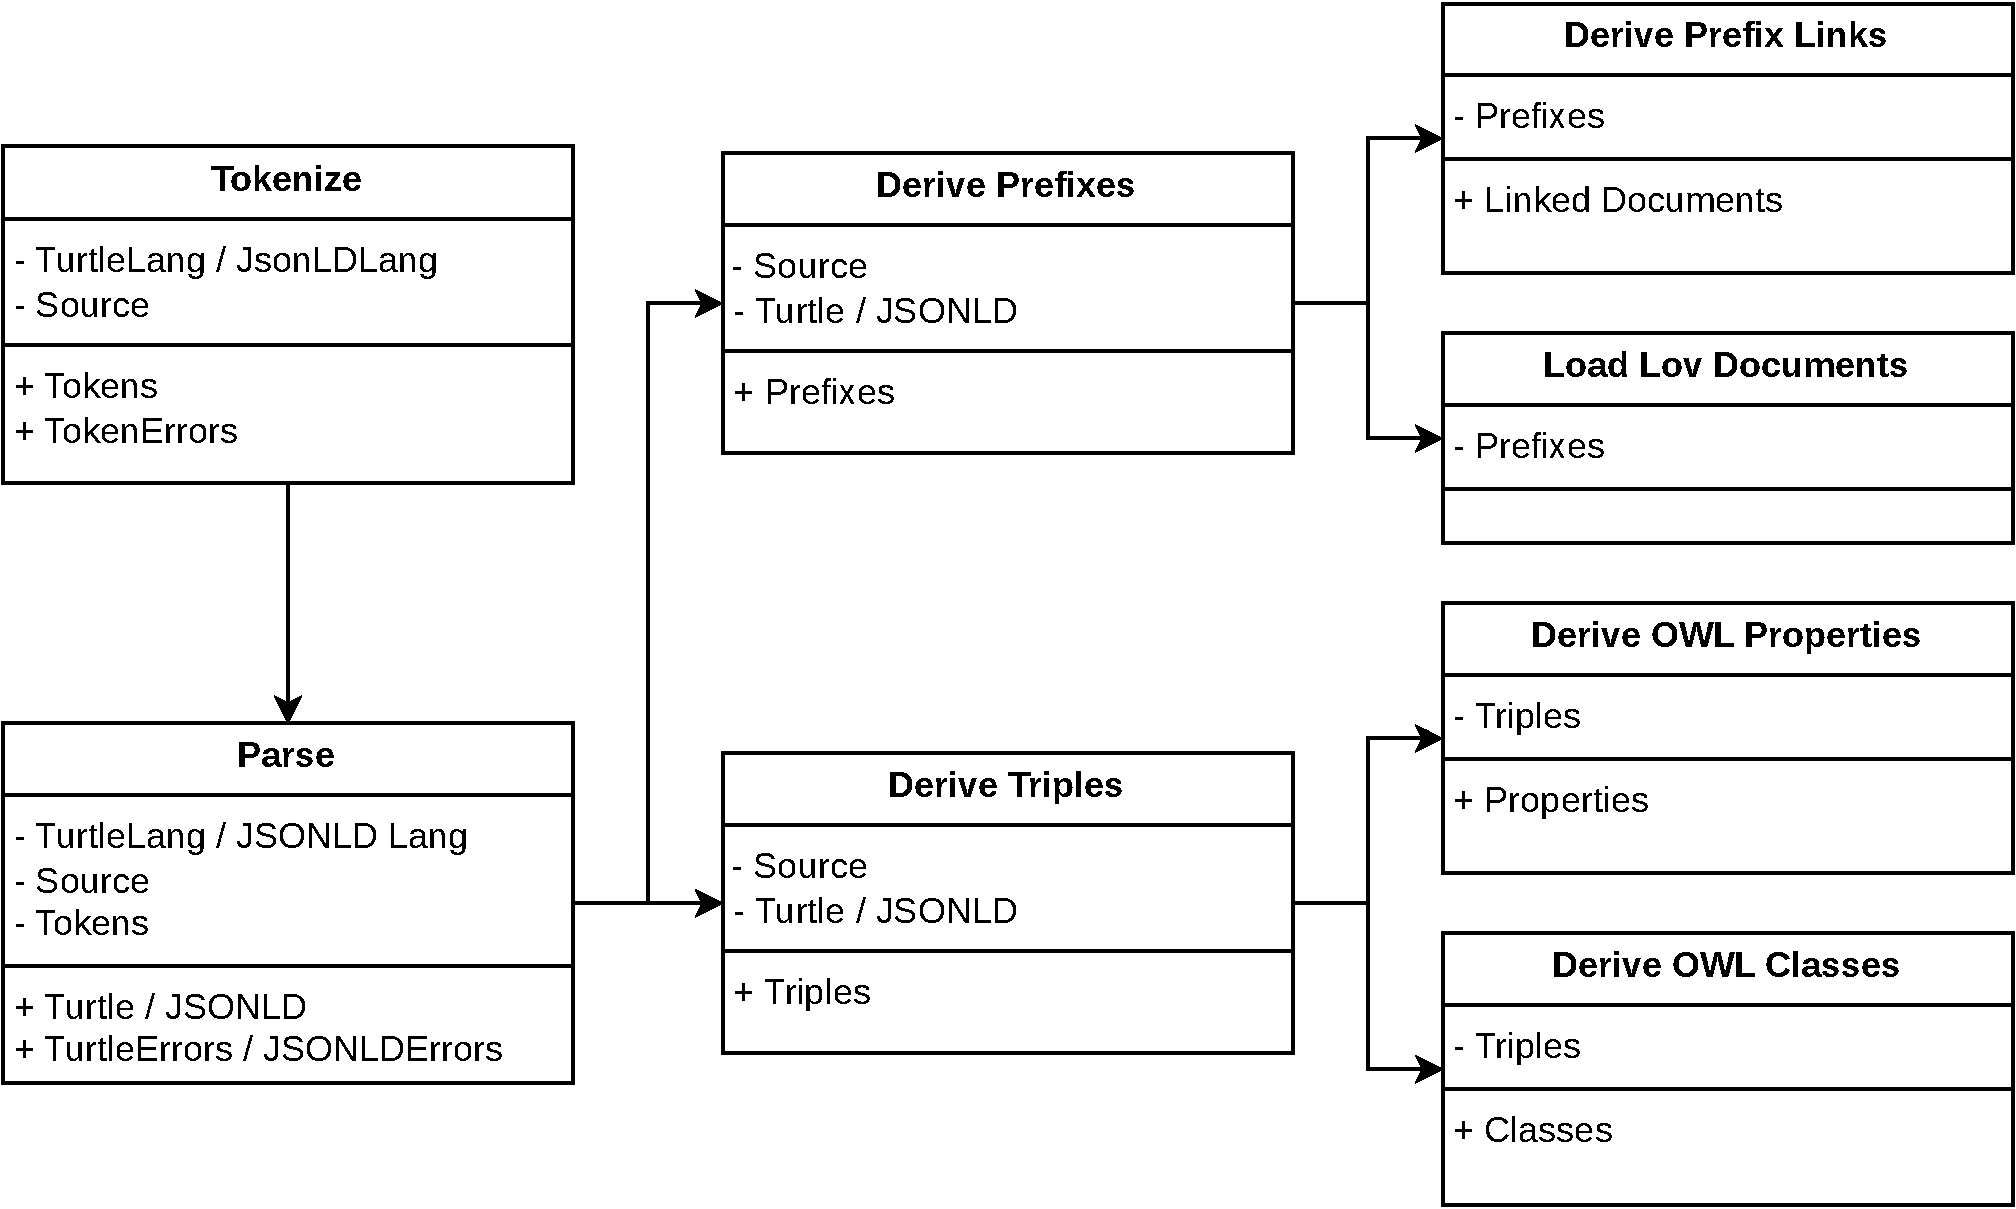
\includegraphics[width=1.2\textwidth]{./images/ParseSchedule.pdf}
 }
  \caption{Visual representation of the Parse schedule including tokenization, parsing, deriving prefixes, deriving triples, linking documents, fetching LOV documents, deriving properties and deriving classes. }\label{fig:Parse}
\end{figure}

The parsing schedule is one of the most important schedules of the language server.
It is activated whenever the user edits a document, the language server is notified with the textual changes.

We chose to let all semantic languages use the same \texttt{token} type, this allows for implementing token based systems only once.
Note that each semantic language does it's own tokenization, not allowing for SPARQL tokens inside Turtle documents.
In Figure \ref{fig:Parse}, \textit{tokenize} is the first sytem in the parsing schedule, this system is implemented for all supported semantic languages. \textit{Tokenize} also report on tokenization errors.

The next system is \textit{parsing}, also implemented for each semantic language, transforming the tokens into actual objects, and reporting on syntactic errors. 
When the objects are parsed, systems are issued that derive prefixes and triples. 
Prefixes contain information about how to expand and shorten iri's for the current document.
Deriving triples does not only derive actual triples, but in the case for SPARQL also bindings, which can be thought of as \textit{triples}.

After deriving prefixes, other systems will create a \texttt{LinkedDocuments} component, listing all documents that are linked some way to this document.
Prefixes are one way, but the object value of the triple \texttt{<> owl:imports <otherLocation>.}, also linkes that other document with the current document.
Prefixes are also used to load the correct LOV defined ontologies, setting up documents containing property and class definitions.

When the triples are derived, a system will derive properties and classes.
In most documents this will result in no properties or classes, but a document linked from LOV will contain many.
The power of the entity component system is that all documents are handled exactly the same.
This allows to cover a use case where a domain expert is writing the ontology and creating SPARQL queries to see how the ontology \textit{feels}, just by importing a local ontology file.

\paragraph{Some words on parsing}

With the language server protocol the server can specify wether or not it requires only the (minimal) changes or entire document every time.
Earlier versions of the semantic lsp required the entire document every time, because documents arae relatively small and reprasing the entire document brings an acceptable performance.
However, we noticed that this hampered the implementation, in turtle specifically there are patterns that cannot be parsed correctly and brings incorrect and frustrating feedback to the user, and partial parsing helps in this regard.
An example is shown in \ref{lst:GroupedListing}.
  The user at \ref{code1} types named node \texttt{<b>}, the language server should not be confused: triple \texttt{<c> <d> <e>} has nothing to do with named node \texttt{<b>}. The language server should suggest objects that fulfill the domain of predicate \texttt{<b>}. 
  The user at \ref{code2} types named node \texttt{<c>}, the language server should not be confused: the are two triples \texttt{<a> <b> <c>} and \texttt{<a> <d> <e>}, however tokenwise the documents are the same. Resulting in the language server suggesting a semi colon.
  
  The user at \ref{code3} just wrote a subject, invocing the subject completion defined in the next section. The language server might incorrect suggest to add a comma after \texttt{<c>} to build a syntactically correct document.
  The user at \ref{code4} is typing a predicate for the subject \texttt{<a>}, the language server might incorrectly parse the document as seen at \ref{code3}, where \texttt{<b>} is subject thus not invocing the property completion as explained in the next section.

  Adding partial parsing eliminates these issues as the language server understand which tokens are new and leaving the original interpretation of the surrounding tokens in touch.


\begin{figure}[tb]
    \centering
    % code1
    \begin{subfigure}{0.21\textwidth}
      \lstinputlisting{./code/option1.ttl}
      \caption{User types \texttt{<b>}}
      \label{code1}
    \end{subfigure}
    \hfill
    % code 2
    \begin{subfigure}{0.21\textwidth}
      \lstinputlisting{./code/option2.ttl}
      \caption{User types \texttt{<c>}}
      \label{code2}
    \end{subfigure}
    \hfill
    % code 3
    \begin{subfigure}{0.21\textwidth}
      \lstinputlisting{./code/option3.ttl}
      \caption{User types \texttt{<a>}}
      \label{code3}
    \end{subfigure}
    \hfill
    % code 4
    \begin{subfigure}{0.21\textwidth}
      \lstinputlisting{./code/option4.ttl}
      \caption{User types \texttt{<b>}}
      \label{code4}
    \end{subfigure}
    \caption{Different code samples showing that it is the indentation/intent of the user that dictates how tokens should be parsed. (a) and (b) show five terms that result in different triples. (c) and (d) show four terms, triples with subject \texttt{<a>} and \texttt{<b>} and both triples with subject \texttt{<a>} resulting in different semantics.    }\label{lst:GroupedListing}
\end{figure}



\subsubsection{Completion}

Completion is one of the most important features that actively interacts with the user.
In the Langauge Server Protocol, the langauge server is issed a completion event that contains the current location of the user.
The server should then answer with a list of completions, including the textual operations, a title and potentially some documentation.
It's the responsibility of the editor to sort and filter the completions and show the user the most relevant information.
How editors do this is not specified, which makes it difficult to create comprehensive testing suite.

\begin{figure}[!ht]
 \centering
 \makebox[\textwidth]{%
    \includegraphics[width=1.2\textwidth]{./images/Completion.pdf}
 }
  \caption{Visual representation of our example pipeline, 
      loading sensor data from The Things Network into a triple store}\label{fig:Completion}
\end{figure}

Figure \ref{fig:Completion} shows a schematic overview of the different systems in the completion schedule and their interactions.
First the server will create a \texttt{CompletionRequest} object, currently containing no completions.
Systems add their relevant completions to the request which is then returned to the user.

The location the user at the moment of the request is not enough information to derive comprehensive completions, 
the first systems will extract more information that is then used by the systems that create the actual completions.

\texttt{GetCurrentToken} expands the current location to the current token, then \texttt{GetCurrentTriple} tries to find the triple that this token corresponds to also indicating whether the user is typing a subject, predicate or object.
If \texttt{GetCurrentToken} fails, the entity lacks a TokenComponent and results in \texttt{GetCurrentTriple} not being issued.

The language server has enough information with only the current token to complete based on defined subjects with the \texttt{SubjectCompletion} system.
The server also completed on already defined prefixes (with \texttt{CompletePrefix}), this system is language agnostic as the Prefixes component is already defined.
To import new prefixes from LOV, each language has to implement a \texttt{CompleteLOVPrefix}, because how to add the import statement is language specific.


\subsubsection{Diagnostics}

The Diagnostics component of the Semantic Language Server (SLS) comprises several focused systems that analyze parsed data to identify issues and provide feedback to users.
Diagnostics differ fundamentally from other language server functionalities because they are push-based: the server actively notifies the editor of errors and warnings.
This allows for timely feedback, ensuring that users can quickly identify and address problems in their semantic documents.

Diagnostics are triggered with two different schedules: on edit and on save.

\begin{enumerate}
  \item \textit{On edit} diagnostics provide fast, real-time feedback to users, enabling them to fix errors as they type. 
    This ensures a fluid editing experience and minimizes interruptions.
  \item \textit{On save} diagnostics occur less frequently and are therefore better suited to more computationally intensive checks,
   such as validation against SHACL shapes.
\end{enumerate}

To demonstrate the capabilities of the diagnostics system, we highlight three key systems:

\begin{enumerate}
  \item \textit{Syntax Diagnostics:}
    During the tokenization and parsing phases, errors such as syntax mismatches or malformed input are detected and recorded, along with their locations.
    These errors are immediately passed to the diagnostics publisher resource, making this part of the on edit schedule, as the necessary data is already generated during parsing.
  \item \textit{SHACL Validation:} 
    With the on save schedule, the server uses the Rudof library to validate the current document against SHACL shapes.
    Shapes are dynamically extracted from the document itself, as well as from prefix links and owl:imports statements.
    This system ensures that the semantic data conforms to expected structural and logical constraints, enabling robust validation for ontologies and linked data documents.
  \item \textit{Basic Validation:}
    This system identifies common issues, such as undefined prefixes or unused declarations.
    By flagging such problems, it helps users maintain consistency and avoid errors that might lead to interoperability issues.
\end{enumerate}

Together, these systems provide comprehensive diagnostic support, catering to both immediate feedback needs and more in-depth validation processes.
This modular approach ensures that diagnostics remain lightweight yet powerful, accommodating the diverse requirements of semantic web practitioners.

\subsubsection{Varia}

Beyond core functionalities, the Semantic Language Server (SLS) offers additional schedules that enhance the user experience and round out its capabilities.
These schedules are smaller in scope, generally focusing on presentation or user interaction rather than deriving new information.

The most notable are as follows:
\begin{enumerate}
  \item \textit{Formatting:}
    A consistent document structure improves readability and reduces the cognitive load required to parse data visually.
    As a formatter, the language server ensures uniformity across documents, promoting best practices and easing collaboration.
    Currently, the SLS includes an opinionated formatter for Turtle, which automatically applies a standardized layout to documents.

  \item \textit{Hover:}
    Hover functionality provides contextual insights about symbols in the document, offering users additional information without disrupting their workflow,
    allowing for users to explore semantic relationships and documentation seamlessly.
    The SLS’s hover implementation includes three key features:
    \begin{itemize}
      \item Type Information: For a node with an inferred type, the hover popup displays the type alongside its hierarchy, including subclasses and superclasses.
      \item Class Details: Hovering over a class reveals its \texttt{rdfs:description}.
      \item Property Insights: Hovering over a property shows its \texttt{rdfs:description}, as well as its range and domain.
    \end{itemize}

  \item \textit{Highlighting:}
    Highlighting improves document readability by visually distinguishing between elements.
    The SLS implements both syntax highlighting and semantic highlighting through a two-step process:
        An initial system maps all tokens to their basic semantic types.
        Subsequent systems refine the types based on additional information.
    For example, in JSON-LD, all keys are initially highlighted as strings.
    However, keys starting with the \texttt{@} symbol are reclassified as keywords, enhancing clarity and usability for JSON-LD documents.
\end{enumerate}

These schedules, while smaller in scale, significantly enhance the language server’s utility by making semantic documents more intuitive and easier to work with.
They represent the \textit{polish} that transforms SLS into a complete tool for semantic web practitioners.



\section{Usage and Potential Impact Across User Groups}%
\label{sec:usage}

This section explores how the Semantic Web Language Server (SWLS) can be used and the expected impact it has across different user groups.
As a language server, SWLS provides functionality that is independent of specific editors, making it highly versatile.
Some editors, such as NeoVim, treat language servers as first-class citizens, offering seamless integration.
Others, like Visual Studio Code and Monaco, require additional glue code to enable effective interaction.
Regardless of the editor, SWLS delivers a consistent set of features that enhance the user experience across all supported platforms.

All code is under a MIT licence available on github\footnote{\url{https://github.com/ajuvercr/semantic-web-lsp}}.
There are currently three ways to interact with SWLS:
\begin{enumerate}
  \item Download the VSCode extension from the market place\footnote{\url{https://marketplace.visualstudio.com/items?itemName=ajuvercr.semantic-web-lsp}}.
  \item Download and compile the binary locally and integrate it into NeoVim\footnote{Installation instruction are available in the README \url{https://github.com/ajuvercr/semantic-web-lsp}}.
  \item Go to the only demo available on \url{https://swls.ajuvercr.be}.
\end{enumerate}

\todo{Maybe add a screenshot of the editors}
In the demo, users are presented with four distinct editors, each tailored to a specific use case.
A toy ontology and its accompanying SHACL shapes serve as foundational resources for the other editors.
One editor is designed for creating small sample data based on the toy ontology, allowing users to explore how semantic concepts can be applied in practice.
Another editor showcases a simple SPARQL query, which, when executed, provides insights derived from data structured according to the ontology.
This setup allows users to immerse themselves in different personas, gaining hands-on experience with various aspects of semantic data workflows.

While all editors, except for the SPARQL editor, are functionally the same, 
the visual seperation improves the realism of the tasks at hand.
Below, we discuss how SWLS benefits each user group and validate its utility in practice.

We first go over the key ways the SWLS might help users, then we will apply these ways to the different user groups defined in Section \ref{sec:introduction}, 
and how those users groups are theorectially assisted by the SWLS.

\subsection{Key Improvements by SWLS}

The SWLS significantly enhances development efficiency by incorporating robust autocompletion features, shown in Figure \ref{class_completion} and Figure \ref{property_completion}.
These features streamline the creation of semantic documents, enabling users to work faster and with fewer errors. 
Whether defining ontologies, creating SHACL shapes, or writing SPARQL queries, the ability to suggest appropriate classes and properties reduces repetitive tasks and minimizes the cognitive load on users, allowing them to focus on the substance of their work.
Autocompletions also helps user explore the current domain by providing context-aware suggestions.

SWLS also aims to improve comprehension by offering real-time feedback on semantic data.
The hover feature (shown in Figure \ref{hover}), which displays detailed information such as associated classes, allows users to quickly grasp the structure and relationships within a document. 
This instant access to contextual information reduces the need for external references and improves overall productivity.

Finally, SWLS aims to increase user confidence in both syntax and semantics
Syntax validation ensures that documents adhere to the expected standards, catching common mistakes as they occur. This feature is shown in Figure \ref{undefined_prefix}.
For semantic validation, the server highlights SHACL violations, helping users align their documents with structural and logical constraints, shown in Figure \ref{shacl_validation}. 
These validation features not only enhance document quality but also provide educational feedback, aiding users in their journey to master semantic web technologies.

\begin{figure}[h!tb]
    \centering
    % code1
    \begin{subfigure}{0.48\textwidth}
      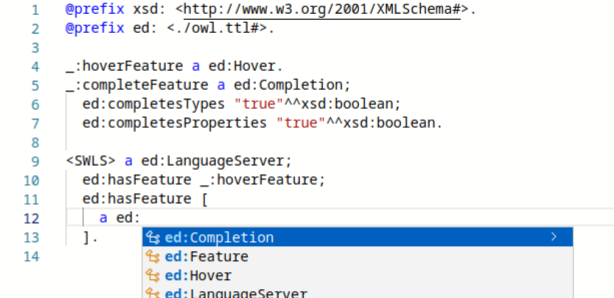
\includegraphics[width=\textwidth]{./images/class_complete.png}
      \caption{SWLS completes a class when the user want to specify the class}
      \label{class_completion}
    \end{subfigure}
    \hfill
    % code 2
    \begin{subfigure}{0.48\textwidth}
      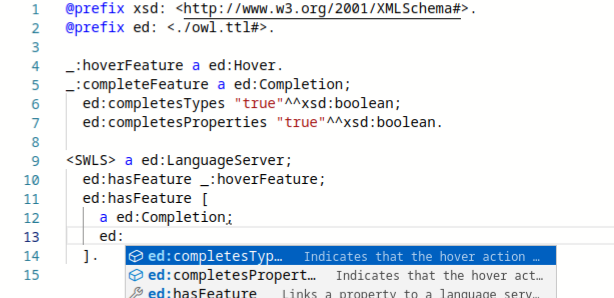
\includegraphics[width=\textwidth]{./images/property_complete.png}
      \caption{SWLS completes properties, first the properties with the correct domain}
      \label{property_completion}
    \end{subfigure}
    \hfill
    % undefined prefix
    % \todo{Actually add those screenshots}
    \begin{subfigure}{0.48\textwidth}
      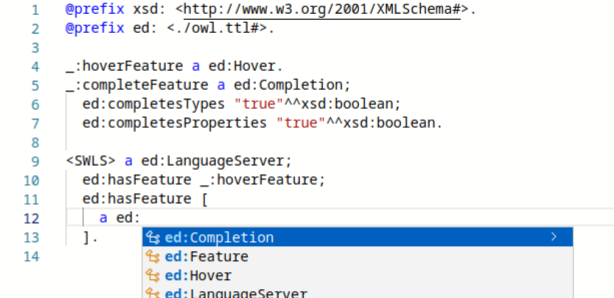
\includegraphics[width=\textwidth]{./images/class_complete.png}
      \caption{SWLS notifies the user of undefined prefixes}
      \label{undefined_prefix}
    \end{subfigure}
    \hfill
    % shacl validation
    \begin{subfigure}{0.48\textwidth}
      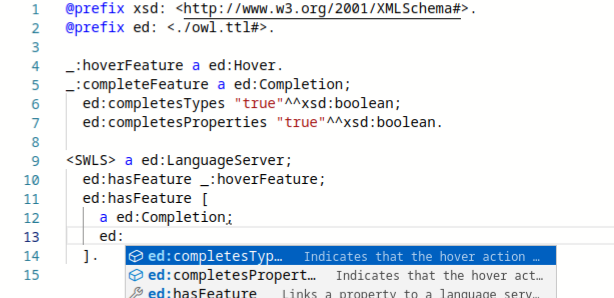
\includegraphics[width=\textwidth]{./images/property_complete.png}
      \caption{SWLS notifies the user of SHACL violations}
      \label{shacl_validation}
    \end{subfigure}
    \hfill
    % shacl validation
    \begin{subfigure}{0.48\textwidth}
      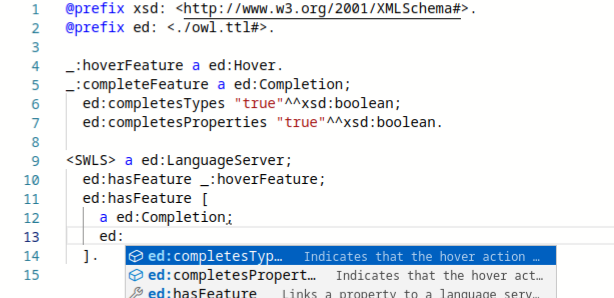
\includegraphics[width=\textwidth]{./images/property_complete.png}
      \caption{SWLS notifies the user of SHACL violations}
      \label{hover}
    \end{subfigure}
    \hfill
    \caption{
      Demo application that shows the usage of SWLS.
      It helps the user by providing autocompletion on classes and properties, taking into account the domain of the properties.
      SWLS also notifies the user of issues like undefined prefixes and SHACL violations.
    }\label{lst:Demo}
\end{figure}

\todo{Add screenshots}

\subsection{User groups}

\paragraph{Semantic power users,} who frequently interact with semantic web technologies, rely on their deep understanding of common properties and domain-specific knowledge to navigate tasks efficiently.
SWLS enhances their workflows by providing robust autocompletion features that streamline document creation and reduce repetitive tasks.
For these users, SWLS also offers a valuable tool for exploring new domains through property suggestions, enabling them to adapt to unfamiliar contexts more easily. 
Additionally, the language server supports quality assurance by helping power users identify common pitfalls such as punning or poorly structured ontologies, ensuring their semantic documents are both accurate and high quality.

\paragraph{For newcomers to the semantic web,} engaging with these technologies can be daunting due to challenges with syntax, semantics, and validation. 
SWLS addresses these pain points by providing immediate feedback on syntax errors, which helps users learn the correct structure and prevents frustration.
The autocompletion feature offers guided support by suggesting relevant properties, allowing users to build confidence in creating semantic documents.
Moreover, validation tools play an educational role: newcomers can intentionally trigger SHACL validation errors to understand what constitutes a faulty document,
turning mistakes into valuable learning opportunities.

\paragraph{Domain experts,} a subset of power users, focus on their specialized fields of knowledge. 
While they share many of the same benefits as general power users, they primarily use SWLS to refine ontologies and ensure alignment with domain-specific standards. 
The autocompletion and hover documentation features help domain experts ensure precision and consistency, facilitating the creation of detailed and accurate semantic models tailored to their expertise.

\paragraph{Data engineers,} on the other hand, primarily work with SPARQL queries to extract meaningful insights from semantic data. 
For these users, SWLS provides critical support by offering autocompletion for classes and properties, as well as syntax validation to prevent errors during query formulation. 
These features significantly enhance productivity by reducing the time spent debugging queries and ensuring accurate results. 
By streamlining the querying process, SWLS enables data engineers to focus on deriving insights rather than resolving technical challenges.



\section{Conclusion}%
\label{sec:conclusion}


% \begin{credits}
% \subsubsection{\ackname} A bold run-in heading in small font size at the end of the paper is
% used for general acknowledgments, for example: This study was funded
% by X (grant number Y).
%
% \subsubsection{\discintname}
% It is now necessary to declare any competing interests or to specifically
% state that the authors have no competing interests. Please place the
% statement with a bold run-in heading in small font size beneath the
% (optional) acknowledgments\footnote{If EquinOCS, our proceedings submission
% system, is used, then the disclaimer can be provided directly in the system.},
% for example: The authors have no competing interests to declare that are
% relevant to the content of this article. Or: Author A has received research
% grants from Company W. Author B has received a speaker honorarium from
% Company X and owns stock in Company Y. Author C is a member of committee Z.
% \end{credits}

\bibliographystyle{splncs04}
\bibliography{./bibliography}

\end{document}
